% LaTeX Template for short student reports.
% Citations should be in bibtex format and go in references.bib
\documentclass[a4paper, 11pt]{article}
\usepackage[top=3cm, bottom=3cm, left = 2cm, right = 2cm]{geometry} 
\geometry{a4paper} 
\usepackage[utf8]{inputenc}
\usepackage{textcomp}
\usepackage{graphicx} 
\usepackage{amsmath,amssymb}  
\usepackage{bm}  
\usepackage[pdftex,bookmarks,colorlinks,breaklinks]{hyperref}  
%\hypersetup{linkcolor=black,citecolor=black,filecolor=black,urlcolor=black} % black links, for printed output
\usepackage{memhfixc} 
\usepackage{pdfsync}  
\usepackage{fancyhdr}
\pagestyle{fancy}



\title{Numerisk øving 2 - TFY4165}
\author{Jacob Oliver Bruun og Sondre Klyve}
%\date{}

\begin{document}
\maketitle
\section*{Kort om prosjektet}
Tilnærmingen til dette numeriske prosjektet ble å lage en sammensatt mappe, som til sammen svarer på oppgaven. Alle utregninger blir gjort i kodefilene, der main.py er hovedfilen, mens read\textunderscore data.py hovedsaklig er for å samle dataen på en fornuftig måte. Videre har vi samlet alle resultat i dette PDF-dokumentet, da vi følte det ble noe rotete å bare kjøre kodefilene. Alle figurer som blir generert, ligger under mappen figures. Datasettet vi fikk utdelt ligger under data.

Vi valgte å løse denne oppgaven ved å bruke objektorientert python. Klassen Mass er definert i read\textunderscore data.py, og er konstruert for å holde på data tilsvarende en fil i data-mappen. Videre har den nyttig funksjonalitet, som å regne ut hastighet. Selve oppgavene løses i main.py, ved å importere Mass-klassen, for deretter å lage spesifisert plott og regne ut ønskede verdier.

Merk at alle plot og verdier i dette dokumentet kan hentes direkte ut ved å kjøre koden. Det vil si at alle plottene blir plottet, og alle verdiene blir skrevet ut til konsollen.

\section*{Oppgave a)}
Main-funksjonen i main.py starter med å lese inn de 49 .txt-filene, og lage et Mass-objekt for hver av de. Videre plotter den histogram for hastighetene, samt spredningsplott av posisjon og hastighet.
Først ser vi spredningsplottene. I hastighetsplottet er midlerere hastighet i $x$- og $y$-retning indikert med stiplet rød linje. Vi ser at disse ligger nær null, som indikerer at massene ikke har drift i noen retning.
\begin{center}
  \[
  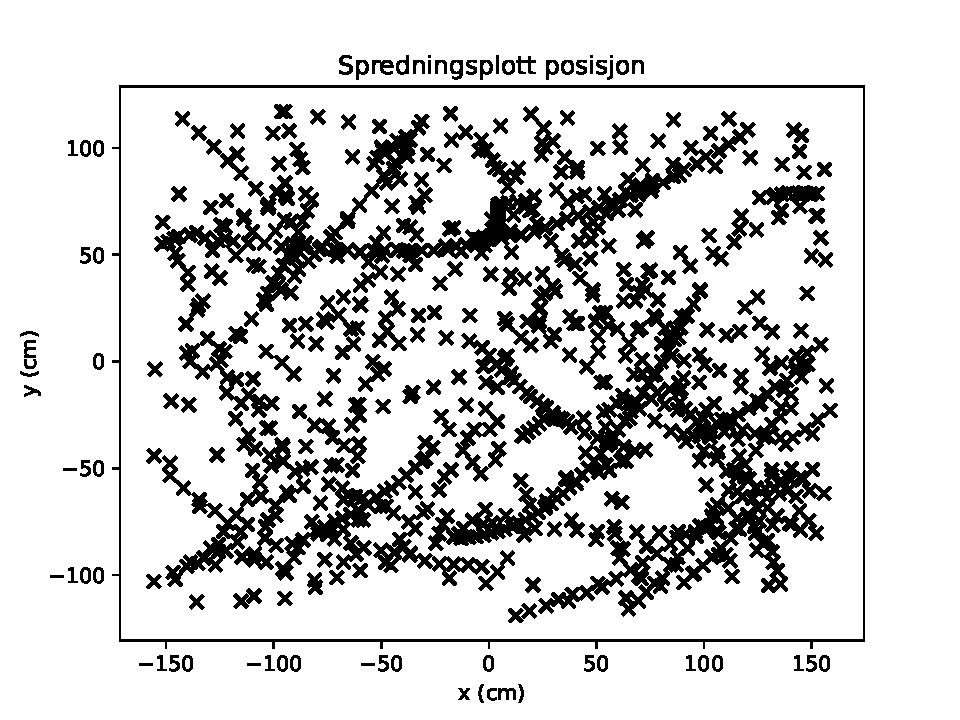
\includegraphics[scale=0.5]{figures/scatterplot_pos.pdf}
  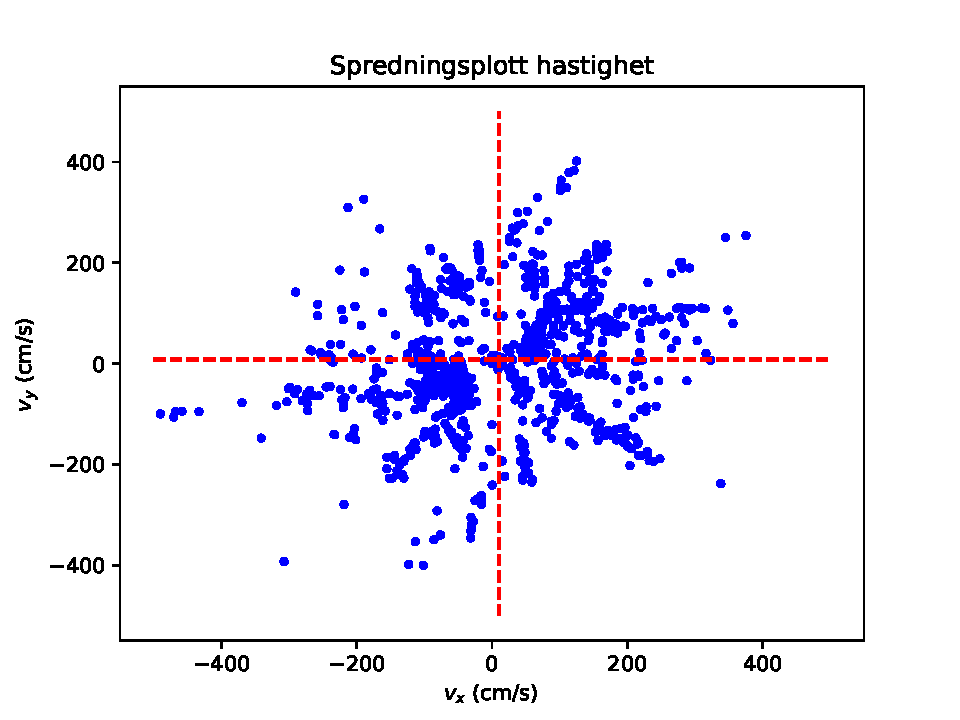
\includegraphics[scale=0.5]{figures/scatterplot_vel.pdf}
  \]
\end{center}
Videre ser vi på histogrammene. Her er den røde linjen teoretisk fordeling. I plottene for $v_x$ og $v_y$, er Maxwells hastighetsfordeling brukt:
\begin{equation}
  g(v_i)dv_i=\sqrt{\frac{B}{\pi}}e^{-Bv_i^2}dv_i\text{  ,  }
  B = \frac{1}{\langle v_i \rangle}.
\end{equation}
\begin{center}
\[
  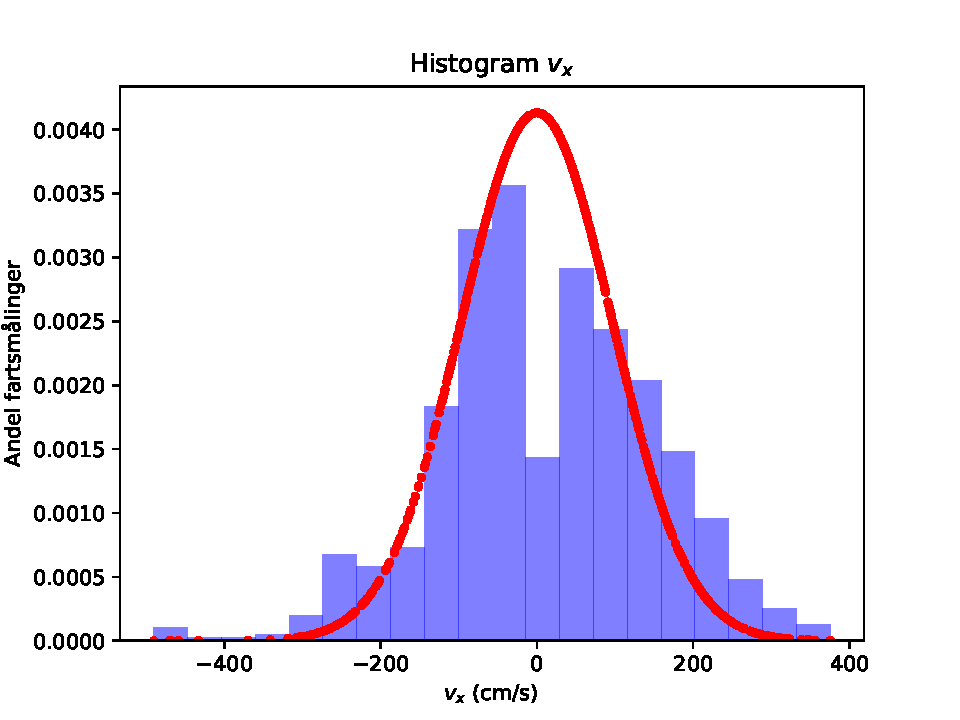
\includegraphics[scale=0.5]{figures/histogram_v_x.pdf}
  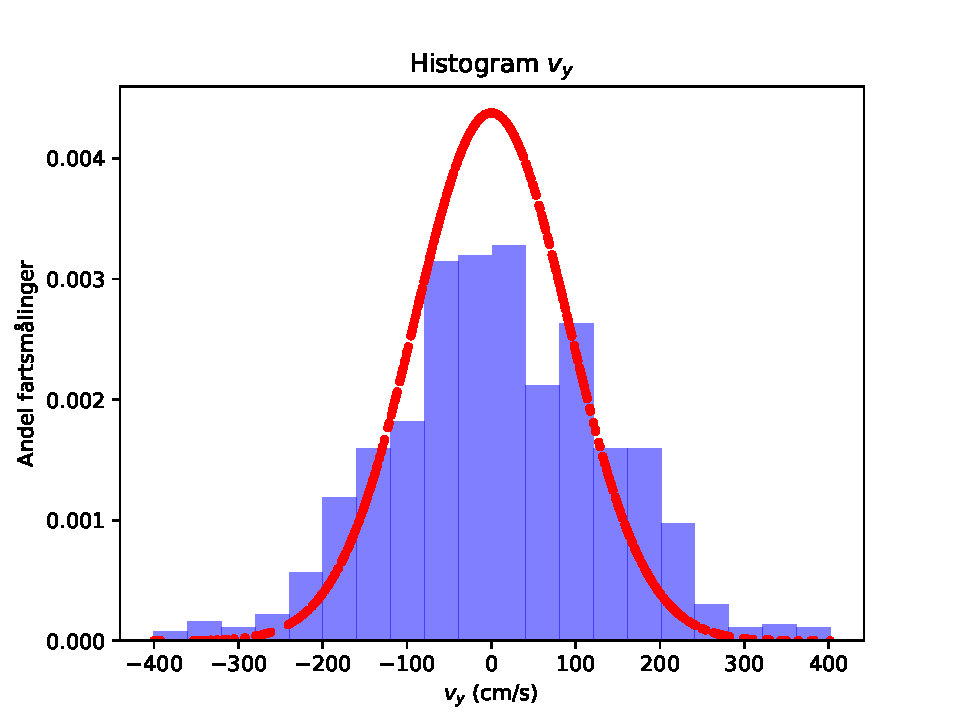
\includegraphics[scale=0.5]{figures/histogram_v_y.pdf}
\]
\end{center}
Fordelingen til $v=\sqrt{v_x^2+v_y^2}$, er fartsfordelingen brukt for å finne teoretisk løsning.
\begin{equation}
  f(v)=2Bve^{-2Bv^2}.
\end{equation}
\begin{center}
\[
  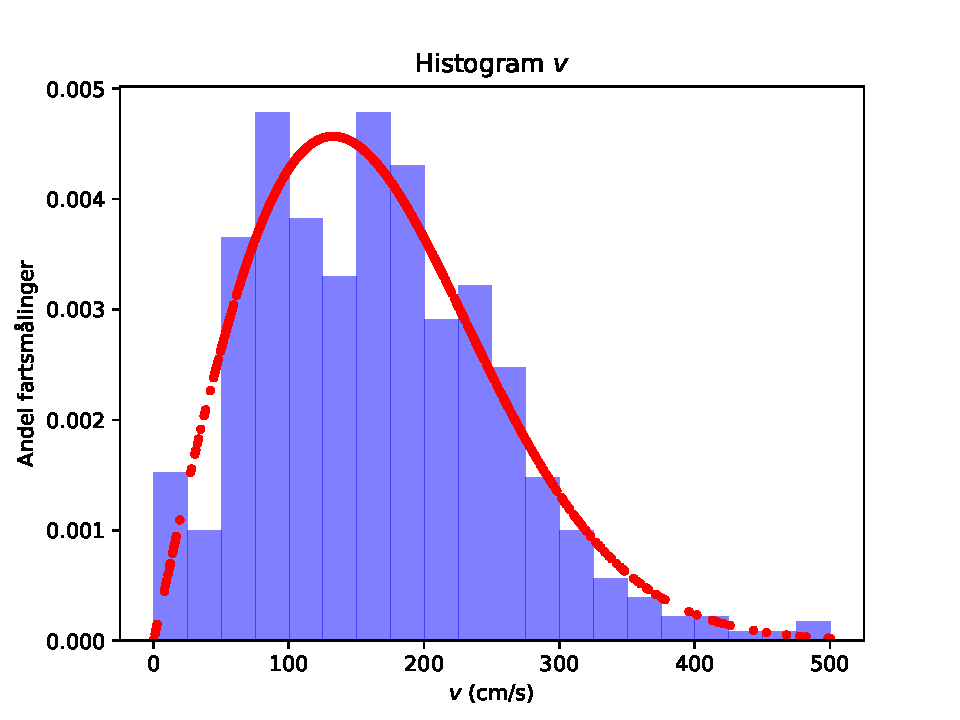
\includegraphics[scale=0.5]{figures/histogram_v.pdf}
\]
\end{center}
Har brukt de oppgitte tipsene, slik at antall intervaller i histogrammene er $N=20$. Histogrammene er også normert ved å bruke density=True i plottefunksjonen.

\newpage
\section*{Oppgave b)}
I funksjonen boltzmann\textunderscore constant regnes ``Boltzmanns plastskivekonstant'' $k_p$ ut for en gitt hastigetsfordeling, samt hvilken temperatur $T$ som måtte til for at en gass skulle oppnå samme hastighetsfordeling som plastskivene i forsøket.
Bruker den oppgitte formelen, og finner da plastskivekonstanten ved
\begin{equation}
  k_p=\frac{m\langle v^2\rangle}{2T}.
\end{equation}
Med oppgitt temperatur $T=300$ K og masse $m=32$ g for plastskivene, får vi plastskivekonstanten
\[
k_p = 1.880 \text{  J}\cdot\text{K}^{-1}
\]
I forhold til Boltzmanns konstant er dette tallet veldig stort, som gir mening med tanke på den store forskjellen i partikkelmasse.

\section*{Oppgave c)}
Regner ut de etterspurte størrelsene.
\begin{table}[h]
  \centering
  \begin{tabular}{|c|c|}
    \hline
    $\langle v \rangle$ & 165.605 cm/s \\
    \hline
    $v_{rms}$ & 187.743 cm/s \\
    \hline
    $\langle v\rangle / v_{rms}$ & 0.882 \\
    \hline
    $\sqrt{\pi}/2$ & 0.886 \\
    \hline
  \end{tabular}
\end{table}
\newline
Ser som forventet at forholdet mellom midlere hastighet og rms-hastighet er nokså lik på $\sqrt{\pi}/2$.

\section*{Oppgave d)}
Som indikert i spredningsplottet til hastighetene, er midlere hastighet for kompnentene nære null, som betyr at vi ikke har betydelig drift i massene.
For sikkerhets skyld regner programmet ut midlere hastigheter, som gir
\begin{align*}
  v_x &= 9.700 \text{cm/s} \\
  v_y &= 8.038 \text{cm/s}.
\end{align*}
Det er ikke helt null, men små i forhold til spennet av hastigheter, som går fra rundt -400 cm/s til 400 cm/s. Dermed går det an å anta at vi har for lite data til å si noe definitivt om det er drift eller ikke. Om dette skulle være et gjengående resultat over flere målinger, vil det være rimelig at det kan være litt drift, for eksempel ved at luftputebordet ikke er helt i vater.
\end{document}